% ============================================================
%  CSE200 Online-1 (A2)  ->  "Fireflies in Unison"
%  Assets in this folder:  fireflies.jpg   firefly_refs.bib
%  Compile:  pdflatex Q3_Fireflies.tex   (twice, for cross-references)
% ============================================================
\documentclass[11pt]{article}

\usepackage[T1]{fontenc}
\usepackage[utf8]{inputenc}
\usepackage[margin=1in]{geometry}
\usepackage{amsmath}
\usepackage{amssymb}
\usepackage{mathtools}          % \boxed etc.
\usepackage{graphicx}
\usepackage{wrapfig}            % figure with text wrapped around it
\usepackage{xcolor}
\usepackage[table]{xcolor}      % \rowcolor for the coloured table (loads colortbl)
\usepackage{booktabs}
\usepackage{array}
\usepackage{enumitem}          % custom list labels
\usepackage{algorithm}
\usepackage{algpseudocode}     % algorithmic pseudo-code
\usepackage{hyperref}

\definecolor{titleblue}{RGB}{40,80,170}
\definecolor{stagered}{RGB}{200,40,40}
\hypersetup{colorlinks=true, linkcolor=titleblue, citecolor=black, urlcolor=titleblue}

\title{\textbf{\textcolor{titleblue}{Fireflies in Unison}}\\[0.3em]
       \large How Simple Timing Rules Create a Collective Rhythm}
\author{Yoshiki Kuramoto\textsuperscript{1} and Steven H. Strogatz\textsuperscript{2}\\[0.3em]
        {\small \textsuperscript{1}Kyoto, Japan \qquad
         \textsuperscript{2}Ithaca, New York, USA}}
\date{}

\begin{document}
\maketitle

% ------------------------------------------------------------
\section{The Puzzle in the Forest}
What do you think happens when hundreds of fireflies gather and begin flashing,
each one following its own slightly different internal clock? At first, the scene
may appear completely random. Yet, after observing and responding to nearby
flashes, the individuals gradually adjust their timing until the entire group
begins to pulse in a shared rhythm---with no leader, no conductor, and no central
control~\cite{sarfati2021}. That's beautiful, right?

This is an example of \emph{synchronization}: interacting systems that initially
behave differently begin to follow a common rhythm. The same broad idea appears in
pendulum clocks, cardiac cells, electrical generators, and communication networks.

\begin{wrapfigure}{r}{0.42\textwidth}
    \centering
    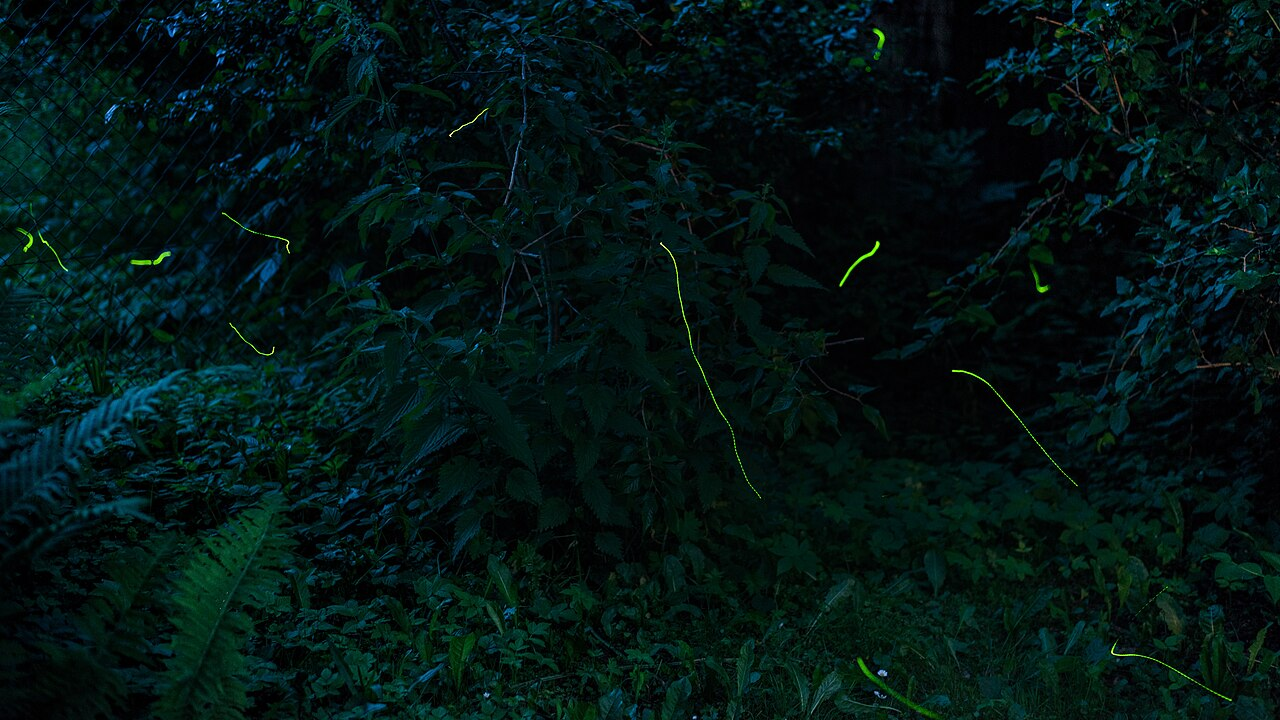
\includegraphics[width=0.40\textwidth]{fireflies.jpg}
    \caption{Firefly light trails in a garden. Photograph by Bernd Thaller, via
             Wikimedia Commons.}
    \label{fig:fireflies}
\end{wrapfigure}

The photograph in fig.~\ref{fig:fireflies} records light trails rather than a
mathematical graph. The model below asks a simpler question:

\begin{quote}\itshape
What is the smallest timing rule that can turn many independent flash cycles into
one coherent display?
\end{quote}

\subsection{A Firefly as a Moving Clock Hand}
Represent firefly $i$ by a phase
\[
    \theta_i(t) \in [0, 2\pi).
\]
One complete trip around the phase circle is one flash cycle. The firefly flashes
when its phase reaches $2\pi$, after which the phase begins again at $0$. If it is
isolated, then
\begin{equation}
    \frac{\mathrm{d}\theta_i}{\mathrm{d}t} = \omega_i, \qquad
    \theta_i(t) = \bigl(\theta_i(0) + \omega_i t\bigr) \bmod 2\pi,
\end{equation}
where $\omega_i$ is its natural angular frequency. A larger $\omega_i$ means a
shorter flash period,
\begin{equation}
    T_i = \frac{2\pi}{\omega_i}.
\end{equation}
Real fireflies emit brief pulses, so this continuous-clock picture is an
approximation.\footnote{Pulse-coupled models represent each flash as a discrete
event and are often closer to the biological mechanism~\cite{mirollo1990}.}

% ------------------------------------------------------------
\section{Listening and Adjusting}

\subsection{The Kuramoto Rule}
A widely used model for interacting phases is
\begin{equation}\label{eq:kuramoto}
    \frac{\mathrm{d}\theta_i}{\mathrm{d}t}
        = \omega_i + \frac{K}{N}\sum_{j=1}^{N}\sin(\theta_j - \theta_i),
        \qquad i = 1,\dots,N.
\end{equation}
The three parts of eq.~\eqref{eq:kuramoto} have direct meanings:
\begin{description}[style=nextline]
    \item[Internal clock] $\omega_i$ is the rate the firefly would follow alone.
    \item[Coupling strength] $K \ge 0$ measures how strongly flashes influence one
          another.
    \item[Timing correction] $\sin(\theta_j - \theta_i)$ tells firefly $i$ whether
          another phase is ahead or behind.
\end{description}

Table~\ref{tab:sine} explains the correction term. The table is simple, but it
contains the central intuition of the model.

\begin{table}[ht]
    \centering
    \caption{How a neighboring firefly affects firefly $i$.}
    \label{tab:sine}
    \begin{tabular}{l l l >{\raggedright\arraybackslash}p{4.3cm}}
        \toprule
        \textbf{Relative position} & \textbf{Phase difference} &
        \textbf{Sine value} & \textbf{Effect on firefly $i$} \\
        \midrule
        \rowcolor{green!10}
        Neighbor ahead  & $0 < \theta_j-\theta_i < \pi$  &
            \textbf{\textcolor{green!55!black}{Positive}} & Speeds up its phase. \\
        \rowcolor{gray!15}
        Phases aligned  & $\theta_j-\theta_i = 0$        &
            \textbf{Zero} & Makes no correction. \\
        \rowcolor{red!10}
        Neighbor behind & $-\pi < \theta_j-\theta_i < 0$ &
            \textbf{\textcolor{red!70!black}{Negative}} & Slows down its phase. \\
        \rowcolor{gray!15}
        Opposite phases & $\theta_j-\theta_i = \pi$      &
            \textbf{Zero} & Produces no preferred direction of correction. \\
        \bottomrule
    \end{tabular}
\end{table}

The sine function is useful because it is smooth, periodic, and changes sign when
the order of two phases is reversed.

% ------------------------------------------------------------
\section{Two Fireflies: An Exact Answer}
The full model may contain hundreds of phases, but the case $N = 2$ can be solved
directly. Define
\[
    \Delta = \theta_2 - \theta_1, \qquad \Delta\omega = \omega_2 - \omega_1.
\]
For two fireflies, eq.~\eqref{eq:kuramoto} becomes
\begin{align}
    \frac{\mathrm{d}\theta_1}{\mathrm{d}t} &= \omega_1 + \frac{K}{2}\sin(\theta_2-\theta_1), \\
    \frac{\mathrm{d}\theta_2}{\mathrm{d}t} &= \omega_2 + \frac{K}{2}\sin(\theta_1-\theta_2).
\end{align}
Subtracting the first equation from the second gives
\begin{align}
    \frac{\mathrm{d}\Delta}{\mathrm{d}t}
        &= \Delta\omega + \frac{K}{2}\sin(-\Delta) - \frac{K}{2}\sin(\Delta) \\
        &= \Delta\omega - K\sin\Delta.
\end{align}
The two fireflies are \emph{phase locked} when $\Delta$ becomes constant. Setting
the left side of eq.~(7) to zero gives
\begin{equation}
    \sin\Delta^* = \frac{\Delta\omega}{K}.
\end{equation}
A real solution exists only when
\begin{equation}
    \boxed{|\Delta\omega| \le K.}
\end{equation}
Thus, coupling can overcome a small mismatch between internal clocks, but not an
arbitrarily large one.

% ------------------------------------------------------------
\section{From a Pair to a Population}

\subsection{Measuring Agreement}
To measure how closely $N$ phases are grouped, define the order parameter
\begin{equation}
    r = \frac{1}{N}\sqrt{\left(\sum_{j=1}^{N}\cos\theta_j\right)^2
                       + \left(\sum_{j=1}^{N}\sin\theta_j\right)^2},
        \qquad 0 \le r \le 1.
\end{equation}
Each phase is treated as a unit arrow. If the arrows point in many directions,
they cancel and $r$ is small. If they point together, they reinforce and $r$
approaches $1$.

As $K$ increases, a typical population passes through three qualitative stages:
\begin{enumerate}[label=\Roman*.]
    \item \textcolor{stagered}{\textbf{Drift:}} phases move mainly according to
          their own natural frequencies.
    \item \textcolor{stagered}{\textbf{Partial locking:}} a group with similar
          frequencies begins to move together.
    \item \textcolor{stagered}{\textbf{Strong coherence:}} most phase differences
          remain bounded and the flashes form a stable rhythm.
\end{enumerate}

% ------------------------------------------------------------
\section{A Short Simulation}
Euler's method can approximate the phase evolution. The following compact
algorithm repeats the interaction and update steps.

\begin{algorithm}[ht]
    \caption{Simulate the Kuramoto model}
    \begin{algorithmic}[1]
        \Require Phases $\theta_i$, frequencies $\omega_i$, coupling $K$, step
                 size $h$, and number of steps $M$
        \For{$m \gets 1$ \textbf{to} $M$}
            \For{each firefly $i$}
                \State $q_i \gets \displaystyle\sum_{j=1}^{N}\sin(\theta_j-\theta_i),
                        \quad v_i \gets \omega_i + \frac{K}{N} q_i$
            \EndFor
            \State Update all phases simultaneously:
                   $\theta_i \gets (\theta_i + h v_i) \bmod 2\pi$
        \EndFor
        \State \Return $\theta_1,\dots,\theta_N$
    \end{algorithmic}
\end{algorithm}

Each firefly compares its phase with all $N$ phases. Therefore, for $M$ time
steps,
\begin{equation}
    T(M,N) = \Theta(MN^2).
\end{equation}

% ------------------------------------------------------------
\section{What the Model Teaches}
The Kuramoto model is deliberately small: it keeps only phase, natural frequency,
and coupling. Yet it explains several general lessons.
\begin{itemize}[label=$\diamond$]
    \item A shared rhythm can emerge without a leader or global clock.
    \item The same mathematical language can describe biological rhythms,
          power-grid generators, chemical oscillations, and distributed timing
          systems.
\end{itemize}
The model also has limitations. Real fireflies interact through visible pulses,
have restricted fields of view, move through space, and may respond differently to
males and females. Those details require richer pulse-coupled or spatial models. A
field study and video of natural synchronous swarms are available through the
\href{https://doi.org/10.1126/sciadv.abg9259}{Science Advances study by Sarfati,
Hayes, and Peleg}.

% ------------------------------------------------------------
%  Bibliography.  The provided firefly_refs.bib can also be used with biblatex:
%     \usepackage[backend=biber,style=numeric]{biblatex}
%     \addbibresource{firefly_refs.bib}   ... \printbibliography
%  The manual list below reproduces the same output and always compiles.
\begin{thebibliography}{9}
\bibitem{sarfati2021}
    Rapha\"el Sarfati, Julie C. Hayes, and Orit Peleg. ``Self-Organization in
    Natural Swarms of \emph{Photinus carolinus} Synchronous Fireflies''. In:
    \emph{Science Advances} 7.28 (2021), eabg9259.
    \textsc{doi}: \href{https://doi.org/10.1126/sciadv.abg9259}{10.1126/sciadv.abg9259}.
\bibitem{mirollo1990}
    Renato E. Mirollo and Steven H. Strogatz. ``Synchronization of Pulse-Coupled
    Biological Oscillators''. In: \emph{SIAM Journal on Applied Mathematics} 50.6
    (1990), pp.~1645--1662.
    \textsc{doi}: \href{https://doi.org/10.1137/0150098}{10.1137/0150098}.
\end{thebibliography}

\end{document}
